\section{Client}
Die Applikation startet mit der Anzeige der untersten Ebene der geladenen Karte (hier Ebene0).
\begin{figure}[H]
\centering
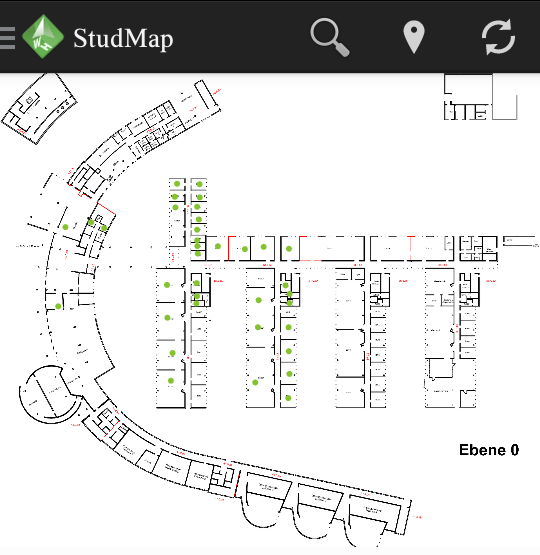
\includegraphics[scale=0.5]{./Bilder/ClientGuide/Start.png}
\caption{Ansicht der App nach erfolgreichem Start}
\label{fig:Startansicht}
\end{figure}

\subsection{Karte}
Die Karte wird �ber verschiedene Touch-Funktionen bedient. So kann mit der bekannten "`Pitch and Zoom Geste"' in die Karte hinein gezoomt werden.
\begin{figure}[H]
\centering
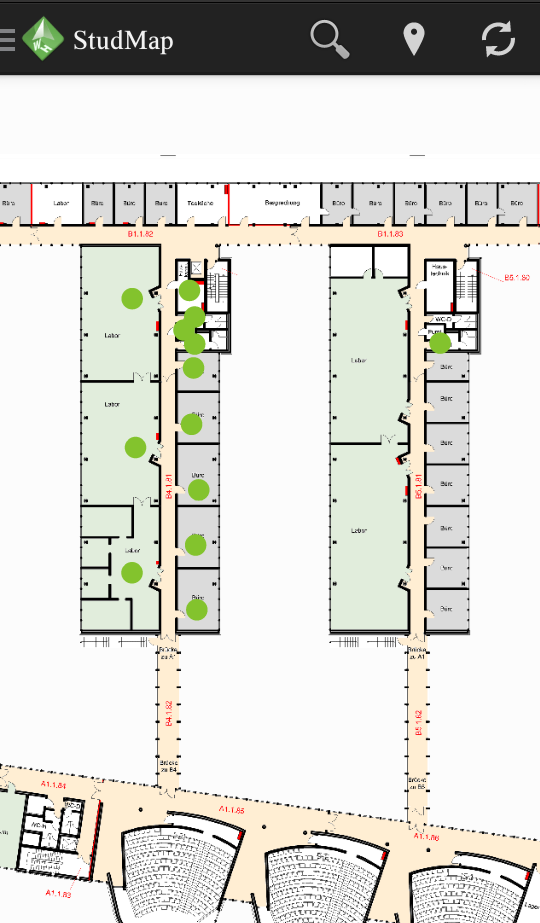
\includegraphics[scale=0.5]{./Bilder/ClientGuide/ZoomEbene1.png}
\caption{Vergr��erte Ansicht von Ebene 1}
\label{fig:ZoomEbene1}
\end{figure}

\subsubsection{Start-/Zielpunkt w�hlen}
\label{ssec:StartZielpunkt}
Um einen Punkt als Start- oder Zielpunkt zu markieren �ffnet sich nach der Anwahl eines Punktes ein Dialog mit entsprechenden Auswahlm�glichkeiten.
\begin{figure}[H]
\centering
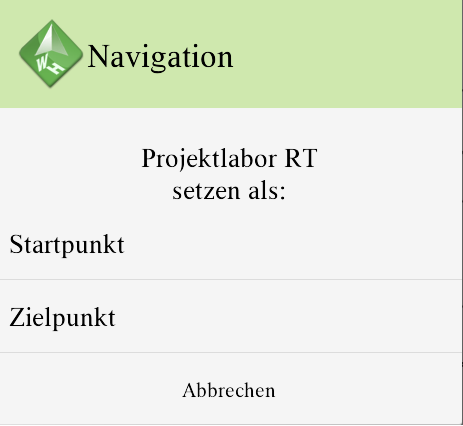
\includegraphics[scale=0.5]{./Bilder/ClientGuide/StartZiel.png}
\caption{Vergr��erte Ansicht des Dialogs zur Entscheidung Start- oder Zielpunkt}
\label{fig:StartZiel}
\end{figure}
Markierte Punkte werden zun�chst auch vergr��ert, rot dargestellt. Der eingeblendete Dialog am Boden der Karte ist jedoch leicht ver�ndert.
\begin{figure}[H]
\centering
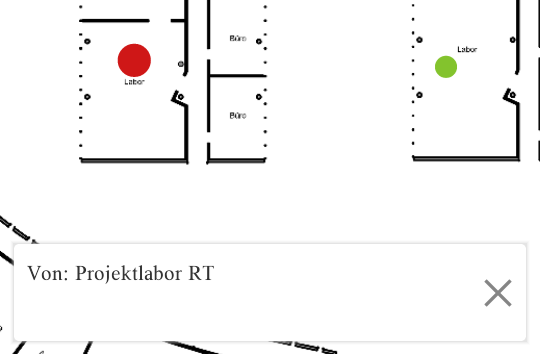
\includegraphics[scale=0.5]{./Bilder/ClientGuide/EinblendungStartpunkt.png}
\caption{Vergr��erte Ansicht des Dialogs f�r einen Startpunkt}
\label{fig:Startpunkt}
\end{figure}

\subsubsection{Navigation}
Wurde ein Start- oder Zielpunkt gew�hlt (siehe \nameref{ssec:StartZielpunkt}), wird der n�chste gew�hlte Punkt automatisch zum Ziel-, bzw. Startpunkt, und eine Route eingezeichnet. Start und Ziel bekommen jeweils ein ansprechendes Symbol und unten im Bild ist eine Einblendung �ber Start und Ziel.
\begin{figure}[H]
\centering
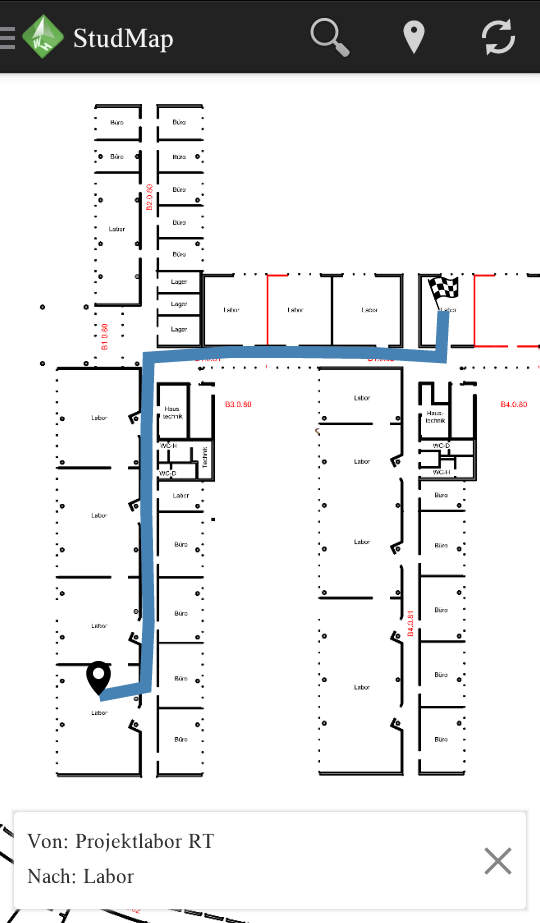
\includegraphics[scale=0.5]{./Bilder/ClientGuide/Navigation.png}
\caption{Ansicht der Karte mit eingeblendeter Route}
\label{fig:Navigation}
\end{figure}

\subsection{ActionBar}
Die Icon in der ActionBar erlauben den Zugriff auf die Suche, die Positionierung und das neu laden der Karte.
\begin{figure}[H]
\centering

\includegraphics[scale=0.7]{./Bilder/ClientGuide/ActionBar.png}
\caption{Vergr��erte Ansicht der ActionBar}
\label{fig:ActionBar}
\end{figure}

\subsubsection{Suche}
Bei der Suchfunktion kann �ber ein Suchfeld, welches sich selbst vervollst�ndigt (\ref{fig:Suchen}, rechtes Bild), ein gesuchter Raum gefunden werden.
\begin{figure}[H]
\centering
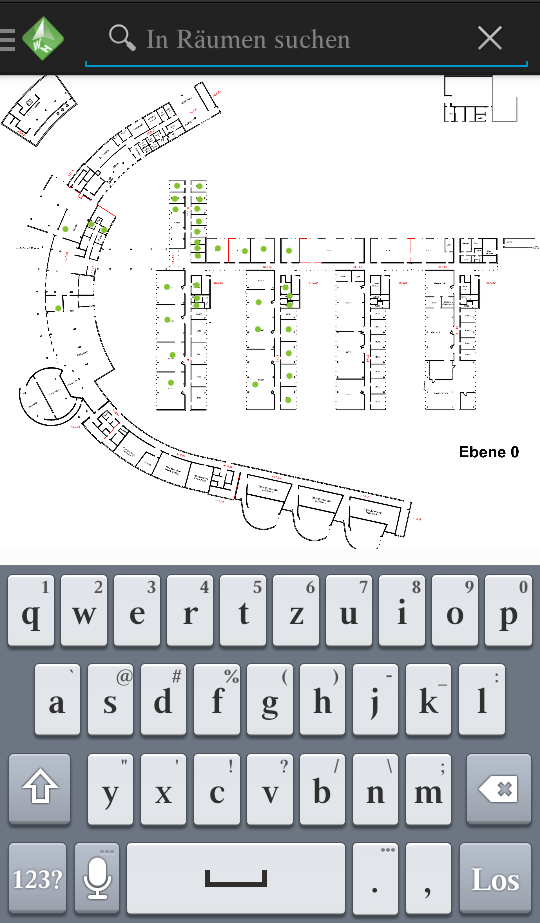
\includegraphics[scale=0.4]{./Bilder/ClientGuide/RaumSuchen.png}
\hspace{15mm}
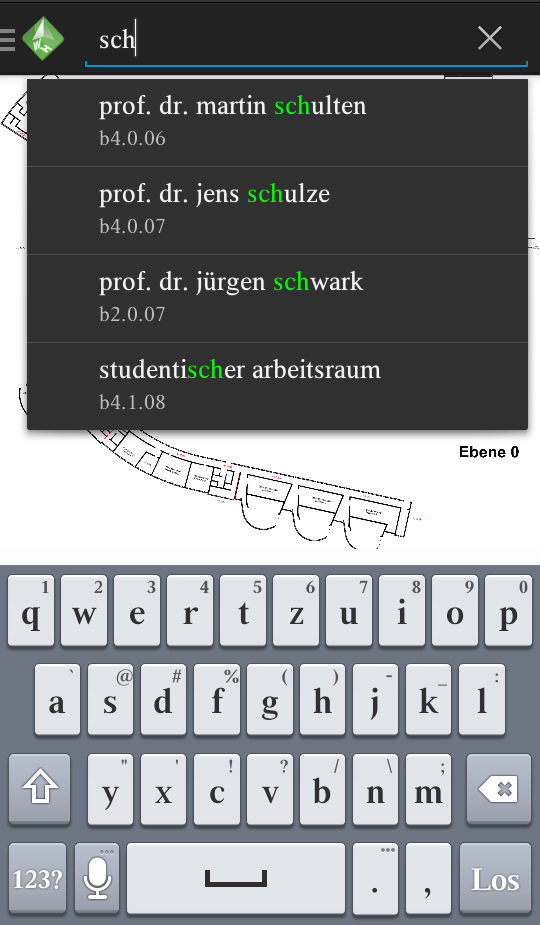
\includegraphics[scale=0.4]{./Bilder/ClientGuide/RaumSuchenAutoComplete.png}
\caption{Ansicht der Suche und der AutoComplete-Funktion}
\label{fig:Suchen}
\end{figure}

Wird ein Punkt durch die Suche, oder auch den PoI-Dialog (siehe \nameref{PoIDialog}) markiert, so wird dieser leicht vergr��ert und rot dargestellt. Im unteren Bildschirm wird zus�tzlich ein Dialog mit den Knoteninformationen eingeblendet.
\begin{figure}[H]
\centering
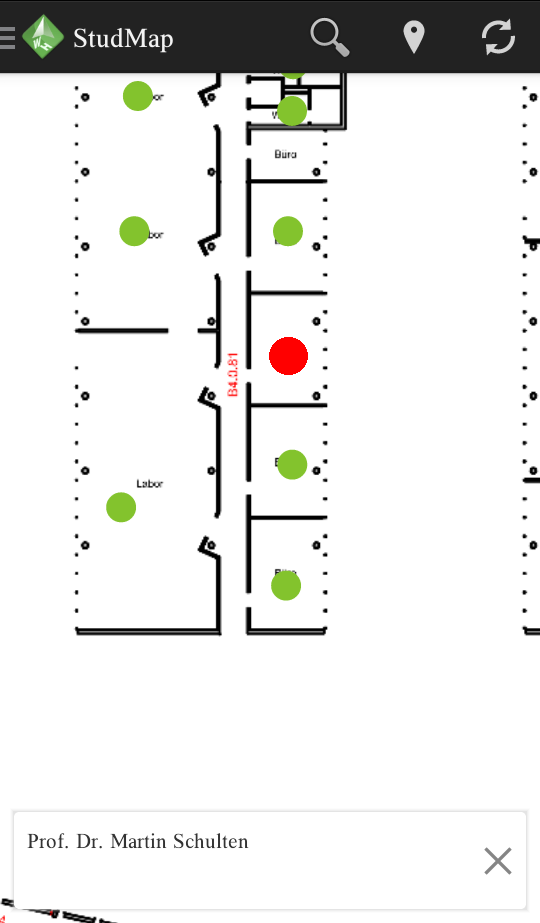
\includegraphics[scale=0.5]{./Bilder/ClientGuide/RaumMarkiert.png}
\caption{Ansicht der Karte mit einem Markierten Raum}
\label{fig:RaumMarkierung}
\end{figure}

\subsubsection{Positionierung}
Die Positionierung kann auf zwei Arten erfolgen. Zum einen kann ein NFC-Tag eingescannt werden, dies erfolgt im Hintergrund und es ist keine Benutzeraktion notwendig. Zum anderen kann ein QR-Tag eingescannt werden, wozu zun�chst �ber das entsprechende Icon der Scanner gestartet werden muss.

\subsubsection{Neu laden}
Sollte die Karte einmal nicht erreichbar sein oder nur fehlerhaft geladen werden, so kann hier das Laden der Karte manuell gestartet werden.

\subsection{Men�}
�ber einen Wisch vom linken Rand nach rechts l�sst sich das Men� aufrufen.
\begin{figure}[H]
\centering
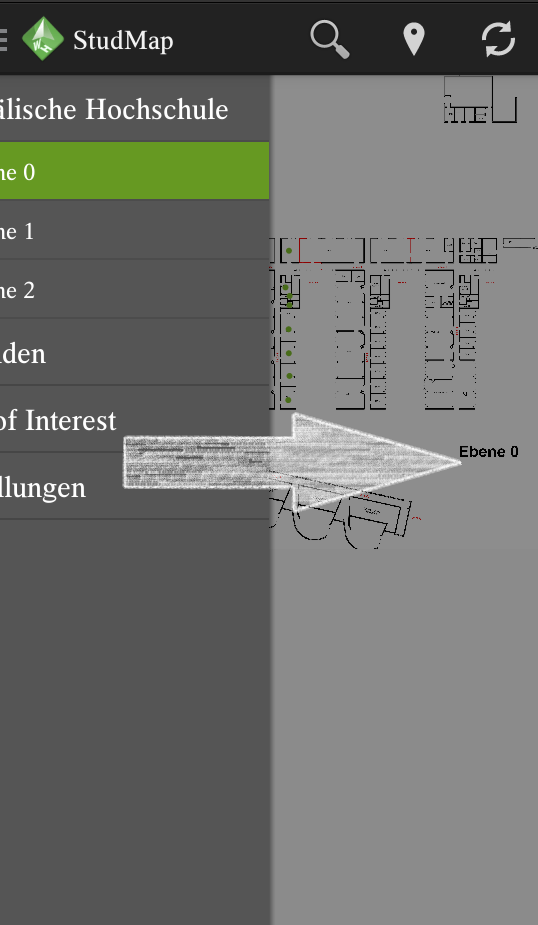
\includegraphics[scale=0.4]{./Bilder/ClientGuide/Swipe.png}
\hspace{15mm}
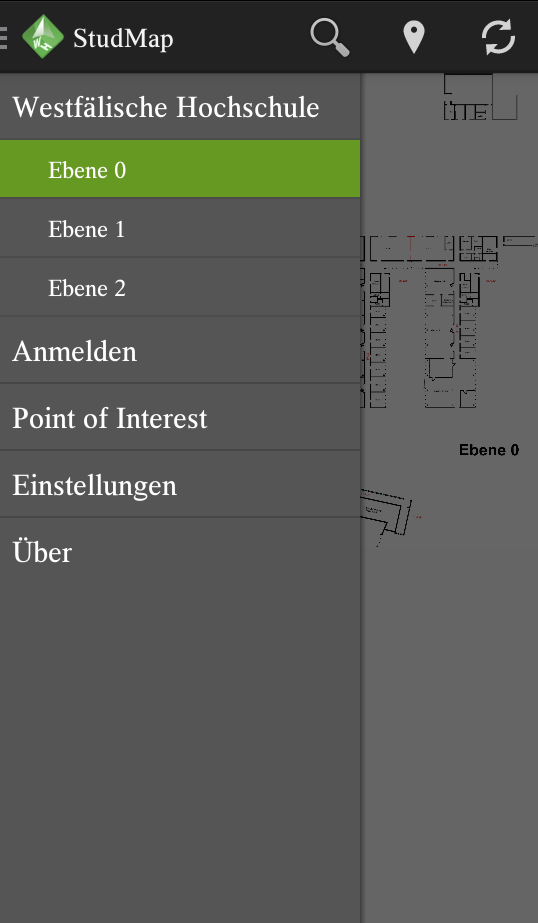
\includegraphics[scale=0.4]{./Bilder/ClientGuide/LeftDrawer.png}
\caption{Ansicht des Men�s}
\label{fig:Menue}
\end{figure}

\subsubsection{Ebene ausw�hlen}
Hier l�sst sich die anzuzeigende Ebene ausw�hlen. Die momentan aktive Ebene wird hellgr�n markiert.
\begin{figure}[H]
\centering
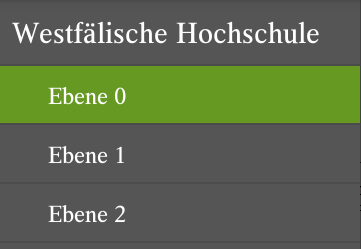
\includegraphics[scale=0.5]{./Bilder/ClientGuide/EbenenAnsicht.png}
\caption{Ausschnitt der Auswahl f�r die Ebenen}
\label{fig:EbenenAnsicht}
\end{figure}

\subsubsection{Anmelden}
In diesem Dialog kann sich der User anmelden erstmalig registrieren.
\begin{figure}[H]
\centering
\includegraphics[scale=0.5]{./Bilder/ClientGuide/AnmeldeDialog.png}
\caption{Ansicht des Dialogs f�r die Anmeldung}
\label{fig:AnmeldeDialog}
\end{figure}

\subsubsection{Point of Interest}
\label{PoIDialog}
Der Dialog gibt einen �berblick �ber interessante Punkte. �ber ein Suchfeld l�sst sich die Auswahl beschr�nken.
\begin{figure}[H]
\centering
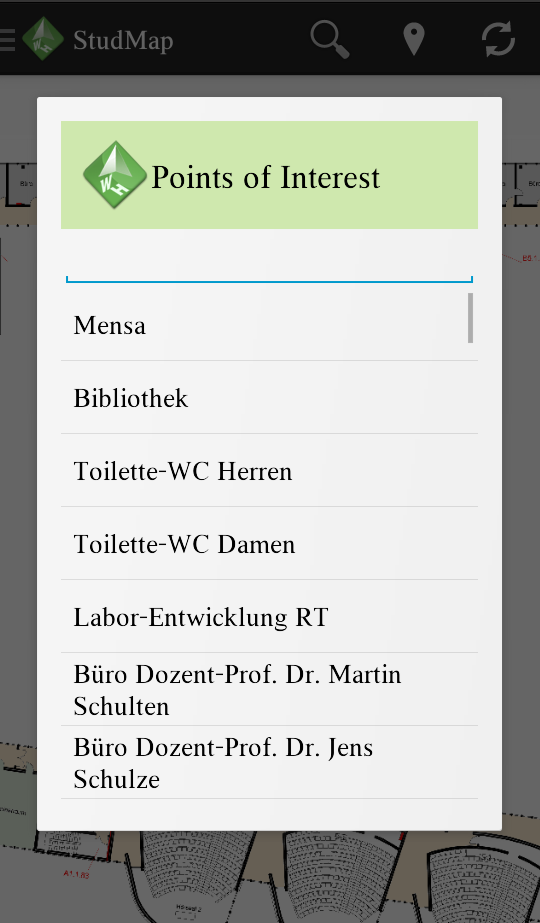
\includegraphics[scale=0.4]{./Bilder/ClientGuide/PoIDialog.png}
\hspace{15mm}
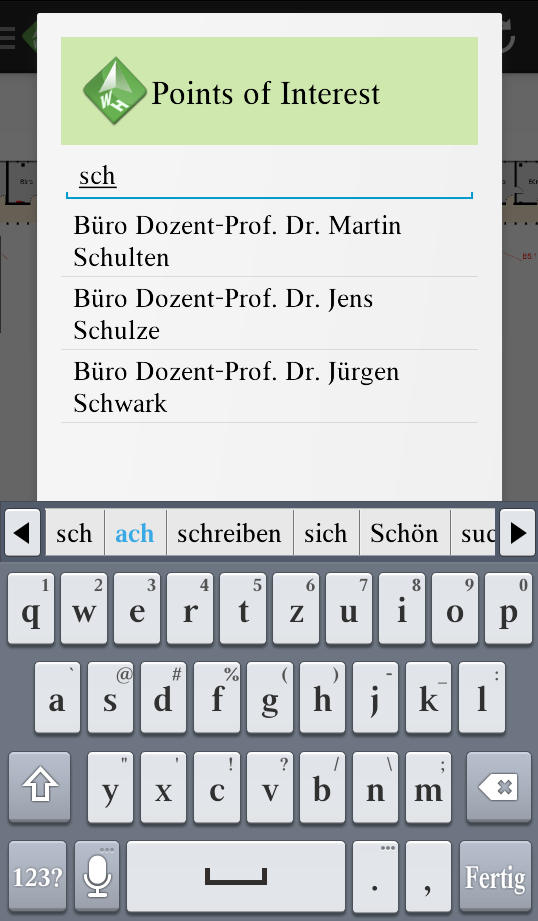
\includegraphics[scale=0.4]{./Bilder/ClientGuide/PoIAutoComplete.png}
\caption{Ansicht des Point of Interest Dialog}
\label{fig:PoIDialog}
\end{figure}

\subsubsection{Einstellungen}
In den Einstellungen k�nnen die anzuzeigende Karte und die IP-Adresse des Host eingestellt, bzw. ge�ndert, werden.
\begin{figure}[H]
\centering
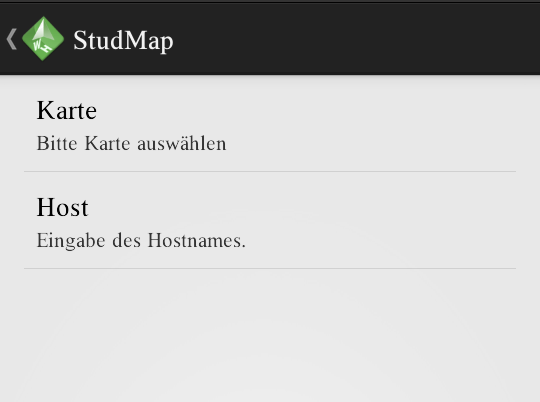
\includegraphics[scale=0.5]{./Bilder/ClientGuide/Settings.png}
\caption{Ansicht der Einstellungen}
\label{fig:Einstellungen}
\end{figure}

\subsubsection{About}
\begin{figure}[H]
\centering
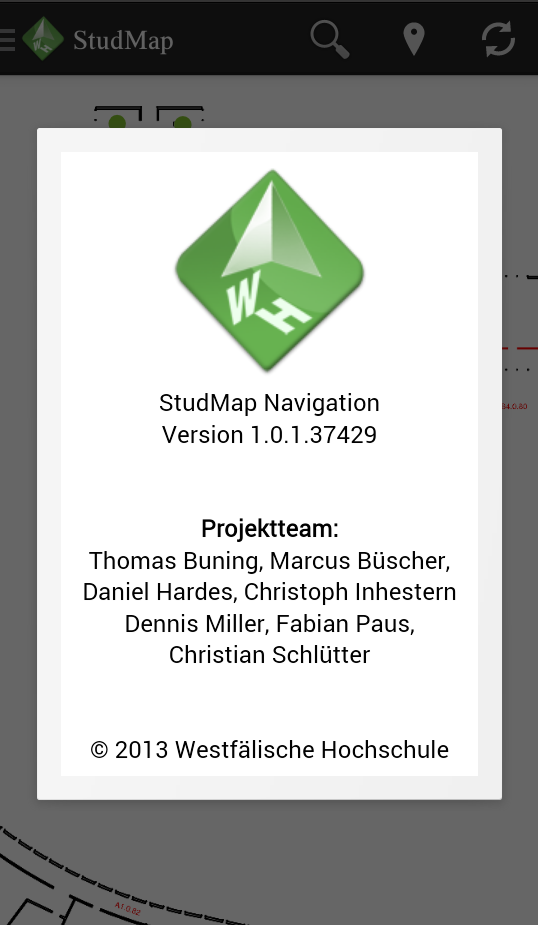
\includegraphics[scale=0.5]{./Bilder/ClientGuide/About.png}
\caption{Ansicht des About Dialogs}
\label{fig:About}
\end{figure}